% Options for packages loaded elsewhere
\PassOptionsToPackage{unicode}{hyperref}
\PassOptionsToPackage{hyphens}{url}
%
\documentclass[
]{article}
\usepackage{amsmath,amssymb}
\usepackage{iftex}
\ifPDFTeX
  \usepackage[T1]{fontenc}
  \usepackage[utf8]{inputenc}
  \usepackage{textcomp} % provide euro and other symbols
\else % if luatex or xetex
  \usepackage{unicode-math} % this also loads fontspec
  \defaultfontfeatures{Scale=MatchLowercase}
  \defaultfontfeatures[\rmfamily]{Ligatures=TeX,Scale=1}
\fi
\usepackage{lmodern}
\ifPDFTeX\else
  % xetex/luatex font selection
\fi
% Use upquote if available, for straight quotes in verbatim environments
\IfFileExists{upquote.sty}{\usepackage{upquote}}{}
\IfFileExists{microtype.sty}{% use microtype if available
  \usepackage[]{microtype}
  \UseMicrotypeSet[protrusion]{basicmath} % disable protrusion for tt fonts
}{}
\makeatletter
\@ifundefined{KOMAClassName}{% if non-KOMA class
  \IfFileExists{parskip.sty}{%
    \usepackage{parskip}
  }{% else
    \setlength{\parindent}{0pt}
    \setlength{\parskip}{6pt plus 2pt minus 1pt}}
}{% if KOMA class
  \KOMAoptions{parskip=half}}
\makeatother
\usepackage{xcolor}
\usepackage[margin=1in]{geometry}
\usepackage{color}
\usepackage{fancyvrb}
\newcommand{\VerbBar}{|}
\newcommand{\VERB}{\Verb[commandchars=\\\{\}]}
\DefineVerbatimEnvironment{Highlighting}{Verbatim}{commandchars=\\\{\}}
% Add ',fontsize=\small' for more characters per line
\usepackage{framed}
\definecolor{shadecolor}{RGB}{248,248,248}
\newenvironment{Shaded}{\begin{snugshade}}{\end{snugshade}}
\newcommand{\AlertTok}[1]{\textcolor[rgb]{0.94,0.16,0.16}{#1}}
\newcommand{\AnnotationTok}[1]{\textcolor[rgb]{0.56,0.35,0.01}{\textbf{\textit{#1}}}}
\newcommand{\AttributeTok}[1]{\textcolor[rgb]{0.13,0.29,0.53}{#1}}
\newcommand{\BaseNTok}[1]{\textcolor[rgb]{0.00,0.00,0.81}{#1}}
\newcommand{\BuiltInTok}[1]{#1}
\newcommand{\CharTok}[1]{\textcolor[rgb]{0.31,0.60,0.02}{#1}}
\newcommand{\CommentTok}[1]{\textcolor[rgb]{0.56,0.35,0.01}{\textit{#1}}}
\newcommand{\CommentVarTok}[1]{\textcolor[rgb]{0.56,0.35,0.01}{\textbf{\textit{#1}}}}
\newcommand{\ConstantTok}[1]{\textcolor[rgb]{0.56,0.35,0.01}{#1}}
\newcommand{\ControlFlowTok}[1]{\textcolor[rgb]{0.13,0.29,0.53}{\textbf{#1}}}
\newcommand{\DataTypeTok}[1]{\textcolor[rgb]{0.13,0.29,0.53}{#1}}
\newcommand{\DecValTok}[1]{\textcolor[rgb]{0.00,0.00,0.81}{#1}}
\newcommand{\DocumentationTok}[1]{\textcolor[rgb]{0.56,0.35,0.01}{\textbf{\textit{#1}}}}
\newcommand{\ErrorTok}[1]{\textcolor[rgb]{0.64,0.00,0.00}{\textbf{#1}}}
\newcommand{\ExtensionTok}[1]{#1}
\newcommand{\FloatTok}[1]{\textcolor[rgb]{0.00,0.00,0.81}{#1}}
\newcommand{\FunctionTok}[1]{\textcolor[rgb]{0.13,0.29,0.53}{\textbf{#1}}}
\newcommand{\ImportTok}[1]{#1}
\newcommand{\InformationTok}[1]{\textcolor[rgb]{0.56,0.35,0.01}{\textbf{\textit{#1}}}}
\newcommand{\KeywordTok}[1]{\textcolor[rgb]{0.13,0.29,0.53}{\textbf{#1}}}
\newcommand{\NormalTok}[1]{#1}
\newcommand{\OperatorTok}[1]{\textcolor[rgb]{0.81,0.36,0.00}{\textbf{#1}}}
\newcommand{\OtherTok}[1]{\textcolor[rgb]{0.56,0.35,0.01}{#1}}
\newcommand{\PreprocessorTok}[1]{\textcolor[rgb]{0.56,0.35,0.01}{\textit{#1}}}
\newcommand{\RegionMarkerTok}[1]{#1}
\newcommand{\SpecialCharTok}[1]{\textcolor[rgb]{0.81,0.36,0.00}{\textbf{#1}}}
\newcommand{\SpecialStringTok}[1]{\textcolor[rgb]{0.31,0.60,0.02}{#1}}
\newcommand{\StringTok}[1]{\textcolor[rgb]{0.31,0.60,0.02}{#1}}
\newcommand{\VariableTok}[1]{\textcolor[rgb]{0.00,0.00,0.00}{#1}}
\newcommand{\VerbatimStringTok}[1]{\textcolor[rgb]{0.31,0.60,0.02}{#1}}
\newcommand{\WarningTok}[1]{\textcolor[rgb]{0.56,0.35,0.01}{\textbf{\textit{#1}}}}
\usepackage{graphicx}
\makeatletter
\def\maxwidth{\ifdim\Gin@nat@width>\linewidth\linewidth\else\Gin@nat@width\fi}
\def\maxheight{\ifdim\Gin@nat@height>\textheight\textheight\else\Gin@nat@height\fi}
\makeatother
% Scale images if necessary, so that they will not overflow the page
% margins by default, and it is still possible to overwrite the defaults
% using explicit options in \includegraphics[width, height, ...]{}
\setkeys{Gin}{width=\maxwidth,height=\maxheight,keepaspectratio}
% Set default figure placement to htbp
\makeatletter
\def\fps@figure{htbp}
\makeatother
\setlength{\emergencystretch}{3em} % prevent overfull lines
\providecommand{\tightlist}{%
  \setlength{\itemsep}{0pt}\setlength{\parskip}{0pt}}
\setcounter{secnumdepth}{-\maxdimen} % remove section numbering
\ifLuaTeX
  \usepackage{selnolig}  % disable illegal ligatures
\fi
\usepackage{bookmark}
\IfFileExists{xurl.sty}{\usepackage{xurl}}{} % add URL line breaks if available
\urlstyle{same}
\hypersetup{
  pdftitle={Written Report - Final Project},
  pdfauthor={Isabella Villanueva},
  hidelinks,
  pdfcreator={LaTeX via pandoc}}

\title{Written Report - Final Project}
\author{Isabella Villanueva}
\date{2024-11-24}

\begin{document}
\maketitle

\subsection{R Markdown}\label{r-markdown}

This is an R Markdown document. Markdown is a simple formatting syntax
for authoring HTML, PDF, and MS Word documents. For more details on
using R Markdown see \url{http://rmarkdown.rstudio.com}.

When you click the \textbf{Knit} button a document will be generated
that includes both content as well as the output of any embedded R code
chunks within the document. You can embed an R code chunk like this:

\begin{Shaded}
\begin{Highlighting}[]
\FunctionTok{summary}\NormalTok{(cars)}
\end{Highlighting}
\end{Shaded}

\begin{verbatim}
##      speed           dist       
##  Min.   : 4.0   Min.   :  2.00  
##  1st Qu.:12.0   1st Qu.: 26.00  
##  Median :15.0   Median : 36.00  
##  Mean   :15.4   Mean   : 42.98  
##  3rd Qu.:19.0   3rd Qu.: 56.00  
##  Max.   :25.0   Max.   :120.00
\end{verbatim}

\subsection{Including Plots}\label{including-plots}

You can also embed plots, for example:

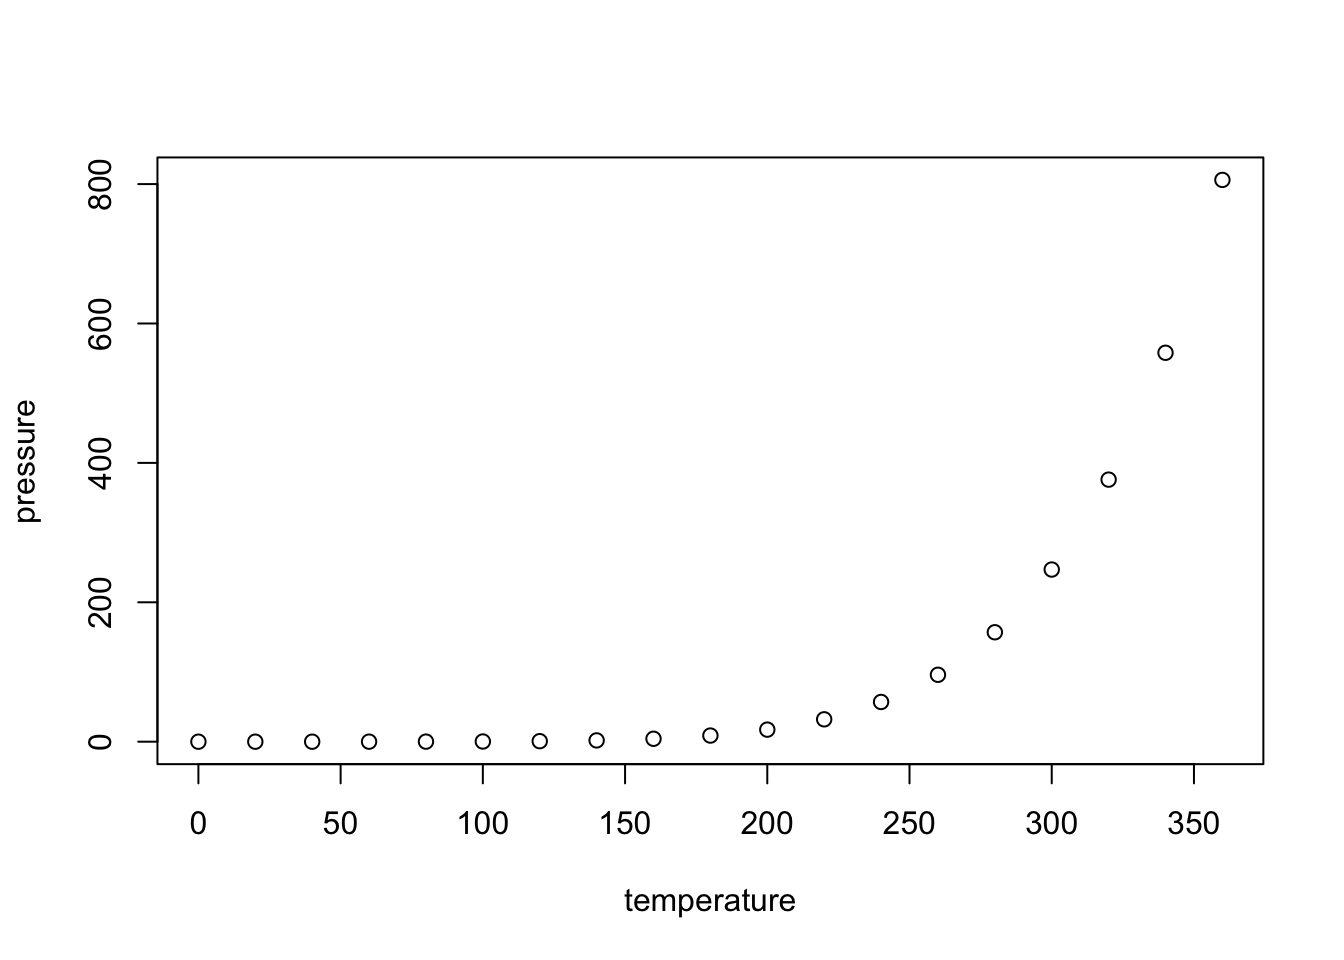
\includegraphics{Written-Report_files/figure-latex/pressure-1.pdf}

Note that the \texttt{echo\ =\ FALSE} parameter was added to the code
chunk to prevent printing of the R code that generated the plot.

\subsection{Introduction}\label{introduction}

In 2023, the opioid crisis was declared a matter of ``national health
emergency''. But the American opioid crisis has been a major public
health issue long before 2023. Marked by a significant rise in drug
poisoning deaths over the past few decades, this epidemic began in the
late 1990s when pharmaceutical companies reassured the doctors and
prescribing health workers that opioid pain relievers were not highly
addictive, leading to widespread over-prescriptions to treat those in
pain. Because of the misinformation about the addictive nature of these
prescription opioids, such as OxyContin and Vicodin, as well as their
increased availability, misuse was inevitable. Over time, patients who
became addicted to prescription opioids often transitioned to cheaper,
more accessible alternatives like heroin and synthetic opioids such as
fentanyl.

By the 2010s, the crisis had escalated. The Centers for Disease Control
and Prevention (CDC) identified three distinct waves of opioid-related
deaths:

\begin{enumerate}
\def\labelenumi{\arabic{enumi}.}
\tightlist
\item
  \textbf{1999--2010}--- Marks the genesis of the opioid crisis with
  rising deaths from prescription opioids
\item
  \textbf{2010--2013} --- A surge in heroin use and overdose deaths as
  access to prescription opioids became restricted
\item
  \textbf{2013- Present} --- The rapid rise of deaths due to illicitly
  manufactured fentanyl (synthetic opioid overdose), which is far more
  potent than heroin or prescription opioids. Yet fentanyl is
  exponentially more dangerous because of its intense potency in small
  quantities -- making it lethal.
\end{enumerate}

National public health agencies, like the CDC, are able to report the
numbers of deaths in the United States because of the death certificate
reporting process, which involves the use of International
Classification of Diseases, Tenth Revision (ICD--10) codes.
``Drug-poisoning deaths are defined as having ICD--10 underlying
cause-of-death codes X40--X44 (unintentional), X60--X64 (suicide), X85
(homicide), or Y10--Y14 (undetermined intent)'' (CDC). According to
National Library of Medicine article ``Defining indicators for drug
overdose emergency department visits and hospitalisations in ICD-10-CM
coded discharge data'', the diagnosis code being used for drug poisoning
cases would begin with the letter T, ``drug poisoning T-codes'' indicate
``poisoning by unspecified drugs, medicaments and biological substances,
accidental (unintentional), initial encounter'' (Vivolo-Kantor et al.).

In the dataset I have chosen: ``Drug Overdose Death Rates by Drug Type,
Sex, Age, Race and Hispanic Origin in the United States (1999 --
2016)'', the CDC reports 2862 observations (rows) of 19 variables
(columns), such as crude and age-related death rates related to drug
poisoning, the states reporting these deaths, and the demographic data
from each individual -- involving salient identity factors like race and
Hispanic origin, sex, and age. These variables will be vital to
exploring which US region has seen the largest influx of drug poisoning
mortality rates in comparison to the US crude rate of drug poisoning
mortality.

\subsubsection{Questions of Interest:}\label{questions-of-interest}

\begin{enumerate}
\def\labelenumi{\arabic{enumi}.}
\item
  Over time (1999-2016) and in consideration of all ages and all
  origins, which regions of the United States have had the greatest
  increase of drug poisoning death rates?
\item
  Throughout the United States, is there a strong association with
  Hispanic origin and drug mortality?
\item
  How do drug poisoning death rates compare between men and women across
  different regions of the U.S. from 1999-2016?
\end{enumerate}

\subsection{Methods}\label{methods}

This public access dataset was created by the National Center for Health
Statistics (NCHS) in December 2017, and available on the CDC Data
website. Among the NCHS content on this database, a plethora of drug
poisoning mortality datasets and visualization tools are available to
assess the opioid crisis under different lenses. For this dataset,
multiple variables of interest were included like sex, age, race and
Hispanic origin, and region. This made this specific dataset the most
attractive because of its amount of information available.

\paragraph{Understanding the NA
Values}\label{understanding-the-na-values}

In cleaning the dataset, checking for NA values is an important step.
Using the function: \texttt{colSums(is.na(drug\_mortality))}, there is
an equal amount of NA values across the variables named
\texttt{Age-adjusted\ Rate},
\texttt{Standard\ Error\ for\ Age-adjusted\ Rate},
\texttt{Lower\ Confidence\ Limit\ for\ Age-adjusted\ Rate},
\texttt{Upper\ Confidence\ Limit\ for\ Age-adjusted\ Rate}. The
age-adjusted rates are missing for many entries, and the decision to
filter them out or use an alternative rate (like crude rates) must be
made.

This equal amount of 1728 NA values is due to how age-adjusted rates
cannot be calculated without the known weight of each age group within a
population each year. When assessing the dataset, the NA values only
occur when matched with the national data (State variable value =
``United States'') as well as the Age Group variable is an age range
rather than ``All Ages''. Because all of the NA values are related to
the age-adjusted rates, this is not an issue for using the data.
Deleting the data with NA values would be a mistake as it augments our
understanding of the true data, and imputing the data to be the mode or
mean of similar characteristics is not possible because it would not be
accurate to what the variables measure.

Crude death rates will be used instead when considering specific age
ranges and when considering the national data, the variable ``US Crude
Rates'' will be used.

\paragraph{Removing Irrelevant
Variables}\label{removing-irrelevant-variables}

Next in cleaning the data, I opted to remove two columns (variables)
because they were not relevant to the data being analyzed. The variable
``Unit'' and ``State Crude Rate in Range'' will not be necessary in this
project because of our intended research question and scope of our data
analysis. The original dataset's Unit variable had two values of
``Deaths per 100,000 resident population, age-adjusted'' or ``Deaths per
100,000 resident population, crude''. The ``Unit'' variable does not
fill any gaps of information that another variable cannot inform, and
removing this variable is not a loss in the greater scope of the data.
The State Crude Rate in Range is not relevant to the question of
interest as we are considering regions in the United States instead of
individual states as well as the comparison to the US Crude Rate, the
State Crude Rate in Range variable is also repetitive and contains
excess information.

After cleaning the data and using the function:
\texttt{str(drug\_mortality{[}sapply(drug\_mortality,\ is.character){]})},
6 variables were loaded in as \texttt{chr} (character or text)
variables: State, Sex, Age Group, Race and Hispanic Origin State Crude
Rate in Range, and Unit have been removed Using the function:
\texttt{str(drug\_mortality{[}sapply(drug\_mortality,\ is.double){]})},
13 variables were loaded in as \texttt{dbl} (double or numeric with
decimal) variables: Year, Deaths, Population, Crude Death Rate, Standard
Error for Crude Rate, Lower Confidence Limit for Crude Rate, Upper
Confidence Limit for Crude Rate, Age-adjusted Rate, Standard Error for
Age-adjusted Rate, Lower Confidence Limit for Age-adjusted Rate, Upper
Confidence Limit for Age-adjusted Rate, US Crude Rate, and US
Age-adjusted Rate

Seeing that the Sex, Race and Hispanic Origin, and Age Group variables
are character or text variables and have repeat values, I decided to
create these variables as factors where repeated values are then
organized into categories (i.e.~Sex has ``Both Sexes'', ``Female'', and
``Male''). This will make calling on these variables in the future
easier, like in the instance of drug mortality rates being compared
between the male and female sexes. Using the function:
\texttt{str(drug\_mortality)} , I was able to authenticate the
conversion of variables to categorical variables where the variables
values were listed by each unique value (i.e.~Sex should only have 3
values if done correctly).

In the case of the variable ``Race and Hispanic Origin'' (RHO), values
like All Races - All Origins, Non-Hispanic Black, Non-Hispanic White,
and Hispanic were all present in this column. To combat the excess of
wordings to get information about this variable, I opted to create a new
categorical variable (new column) named Hispanic and assign values
whether the individual is of Hispanic origin or not. When the RHO column
indicated only the word ``Hispanic'' the value would be 1, while the
value would be 0 if the RHO column indicated ``Non-Hispanic'' along with
their race, or if it indicated ``All Races - All Origins''.

\paragraph{Representative States for US
Regions}\label{representative-states-for-us-regions}

Our research question of interest asks what regions have had the
greatest increase in drug poisoning mortality, I also opted to divide
all 50 states (and the District of Columbia) into their respective US
regions according the
\href{https://www.cdc.gov/nchs/hus/sources-definitions/geographic-region.htm}{how
the CDC defines the geographic regions in the United States}. The
previous use of the representative 5 states for the US regions is
helpful to guide our hypotheses on which regions are expected to have
higher drug poisoning mortality rates, but to get a more specific
visualization of the data, use of all 50 states (and additional
territory of the nation's capital, Washington D.C.) is necessary.

In the State variable, ``United States'' is also included as a value
which indicates that data of those rows are national data, which points
to the US Crude Rates. This will be useful when comparing the regions to
the national rates.

\subsection{Conclusion (include
graphs)}\label{conclusion-include-graphs}

Four graphs were created to visualize the numerical data of the average
drug poisoning mortality rates in each US region and compare these rates
to the national average. When considering the research question of
interest, the US region that has the greatest increase in drug poisoning
mortality in comparison to all US four regions and the national average
was \textbf{the Northeast region}, clearly visualized by the second line
plot graphing ``Average Drug Poisoning Death Rate by US Region
(1999-2016)''.

The initial graph, showing the representative 5 states of each US
region, allows the observers to gain an initial impression of the data.
With this line graph ``Average Drug Poisoning Death Rate by
Representative State'', we notice that Illinois (representing the
Midwest) and New York (representing the Northeast) have the steepest
slopes in this initial line graph, indicating that these two regions may
have the higher mortality rates than the other regions. When allowing
more specificity by dividing all 50 states and the District of Columbia
into the four US regions, we can properly assess the mortality rates of
each region and can conclude that the Northeast region has had the
greatest increase in mortality rates, as indicated by the steep slope of
its line (large increase over smaller period of time) as well as the
magnitude of the mean death rate value (nearing 40 deaths per 100,000 at
the peak in the year 2016). When ranking the steepness of linear slopes
of each region, the South has the second steepest slope, then the
National mortality rate, then the Midwest, and finally the West. The
West region is ranked last in this ranking, though in the graph it has
the third highest mortality rate of about 17 deaths per 100,000 persons,
its slope plateaus around the year 2011-2012, and steadily rises as seen
in the faceted line plot.

The box plot presents similar information in a different format, where
the Northeast, South, and Midwest have similar distributions with some
higher outliers, but the West consistently shows lower mortality rates,
visualized in lowest amount of outliers (even its outliers are lower
than the other 4 categories) as well as a seemingly normal distribution
in its box plot. The Midwest, like the line plots, has the lowest
mortality rates but drastically increases over time. The national
distribution has the largest spread and the highest overall outliers,
reflecting the extreme cases across the U.S.

\subsubsection{Potential Factors Behind Observed
Trends}\label{potential-factors-behind-observed-trends}

Public health responses to the declaration of a national health
emergency have affected populations, yet some regions of the United
States may have more ease of accessing health care arising from policy
like increased regulation of opioid prescriptions, efforts to expand
access to treatment for opioid use disorder, and the distribution of
naloxone --- a life-saving medication that can reverse opioid overdoses.
This may explain the plateau of the West region's drug poisoning
mortality rates, while Northeast and South rates continued to skyrocket
-- as these regions are politically more diverse and unlikely to resolve
policy easily. Despite these efforts, drug poisoning deaths have
continued to rise in the last decade, exacerbated by the increasing
presence of synthetic opioids like fentanyl noted as the ``third wave''
of the opioid epidemic.

The opioid crisis undoubtedly disproportionately affects certain
demographics, with higher rates among middle-aged adults, non-Hispanic
whites, and men. It would be worth exploring the correlation rates
between these demographics, such as sex, Hispanic origin, and age, with
the newfound knowledge gained from this data analysis of US regions and
death mortality rates.

\end{document}
